\documentclass[a4paper, 12pt]{article}
\usepackage{amsmath}
\usepackage{pgfplots}
\usepackage{tabularx}
\usepackage[font=small,labelfont=bf]{caption}

\usepgfplotslibrary{dateplot}

\newcommand{\templates}{../../template}
\usepackage[a4paper, margin=2.5cm]{geometry}

\usepackage{enumitem}
\setlist[itemize]{noitemsep}
\setlist[enumerate]{noitemsep}

\let\oldpar\paragraph
\renewcommand{\paragraph}[1]{\oldpar{#1\\}\noindent}
\usepackage{graphicx}
\usepackage{hyperref}
\usepackage{makecell}

\newcommand{\settitolo}[1]{\newcommand{\titolo}{#1\\}}
\newcommand{\setprogetto}[1]{\newcommand{\progetto}{#1\\}}
\newcommand{\setcommittenti}[1]{\newcommand{\committenti}{#1\\}}
\newcommand{\setredattori}[1]{\newcommand{\redattori}{#1\\}}
\newcommand{\setrevisori}[1]{\newcommand{\revisori}{#1\\}}
\newcommand{\setresponsabili}[1]{\newcommand{\responsabili}{#1\\}}
\newcommand{\setversione}[1]{
	\ifdefined\versione\renewcommand{\versione}{#1\\}
	\else\newcommand{\versione}{#1\\}\fi
}
\newcommand{\setdestuso}[1]{\newcommand{\uso}{#1\\}}
\newcommand{\setdescrizione}[1]{\newcommand{\descrizione}{#1\\}}

\newcommand{\makefrontpage}{
	\begin{titlepage}
		\begin{center}

		
\includegraphics[width=0.4\textwidth]{../../template/WSWS-logos_transparent_crop}\\

		{\Large Winning Software Solution}\\[6pt]
		\href{mailto://winningsoftwaresolution@gmail.com}{winningsoftwaresolution@gmail.com}\\
		
		\ifdefined\progetto
		\vspace{1cm}
		{\Large\progetto}
		{\large\committenti}
		\else\fi
		
		\vspace{1.5cm}
		{\LARGE\titolo}
		
		\vfill
		
		\begin{tabular}{r | l}
		\multicolumn{2}{c}{\textit{Informazioni}}\\
		\hline
		
		\ifdefined\redattori
			\textit{Redattori} &
			\makecell[l]{\redattori}\\
		\else\fi
		\ifdefined\revisori
			\textit{Revisori} &
			\makecell[l]{\revisori}\\
		\else\fi
		\ifdefined\responsabili
			\textit{Respondabili} &
			\makecell[l]{\responsabili}\\
		\else\fi
		
		\ifdefined\versione
			\textit{Versione} & \versione
		\else\fi
		
		\textit{Uso} & \uso
		
		\end{tabular}
		
		\vspace{2cm}
		
		\ifdefined\descrizione
		Descrizione
		\vspace{6pt}
		\hrule
		\descrizione
		\else\fi
		\end{center}
	\end{titlepage}
}
\usepackage{hyperref}
\usepackage{array}
\usepackage{tabularx}

\def\vers#1-#2-#3-#4-#5\\{#1&#2&#3&#4&#5\\\hline}

\newcommand{\addversione}[5]{
	\ifdefined\versioni
		\let\old\versioni
		\renewcommand{\versioni}{#1&#2&#3&#4&#5\\\hline\old}
	\else
		\newcommand{\versioni}{#1&#2&#3&#4&#5\\\hline}
	\fi
}

\newcommand{\setversioni}[1]{\newcommand{\versioni}{#1}}

\newcommand{\makeversioni}{
	\begin{center}
		\begin{tabularx}{\textwidth}{|c|c|c|c|X|}
		\hline
		\textbf{Versione} & \textbf{Data} & \textbf{Persona} & \textbf{Attivtà} & \textbf{Descrizione} \\
		\hline
		\versioni
		\end{tabularx}
	\end{center}
	\clearpage
}

\settitolo{Piano di Qualifica}
\setredattori{Raffaele Oliviero \\ Elia Scandaletti \\ Giovanni Cocco}
\setdestuso{esterno}
\setdescrizione{
Questo documento serve a definire le metriche e i criteri di accettazione dei prodotti.
}

\addversione{0.0.0}{09/01/2022}{Raffaele Oliviero}{Redazione}{Stesura iniziale.}
\addversione{0.0.1}{16/01/2022}{Elia Scandaletti}{Redazione}{Correzione indice di Gulpease.}
\addversione{0.0.2}{16/01/2022}{Giovanni Cocco}{Redazione}{Migliorata la leggibilità.}
\addversione{0.0.3}{04/02/2022}{Giovanni Cocco}{Redazione}{Stesura iniziale sezione software.}
\addversione{0.0.4}{21/02/2022}{Giovanni Cocco}{Redazione}{Aggiunta dashboard al docuemento.}
\addversione{2.0.0}{23/03/2022}{Elia Scandaletti}{Redazione}{Rifacimento del documento.}
\addversione{2.1.0}{30/03/2022}{Giovanni Cocco}{Redazione}{Aggiornamento per ciclo 1.}
\addversione{2.2.0}{07/04/2022}{Matteo Galvagni}{Redazione}{Aggiornamento per ciclo 2.}
\addversione{2.2.0}{13/04/2022}{Federico Marchi}{Redazione}{Aggiornamento per ciclo 3.}

\begin{document}

\makefrontpage

\makeversioni

\tableofcontents
\clearpage

\section{Qualità di prodotto}

\subsection{Documentazione}
\subsubsection{Indice di Gulpease}
\[ \text{Indice di Gulpease} = 89 + \frac{300*\text{\#frasi} - 10*\text{\#lettere}}{\text{\#parole}} \]
\begin{itemize}
	\item \#lettere: numero di caratteri alfanumerici;
	\item \#parole: numero di gruppi di caratteri alfanumerici;
	\item \#frasi: numero di gruppi di punti o punti e virgola consecutivi.
\end{itemize}

\subparagraph{Prodotti coinvolti:}
\begin{center}
	\begin{tabularx}{\textwidth}{|X|X|X|}
		\hline
		\textbf{Prodotto} & \textbf{Valore accettabile} & \textbf{Valore ottimale } \\
		\hline
		Documenti interni & $>$ 40                      & $>$ 50                    \\
		\hline
		Documenti esterni & $>$ 40                      & $>$ 60                    \\
		\hline
	\end{tabularx}\\[8pt]
	\mbox{}\\
\end{center}
\subparagraph{Note:}
Si tiene conto che un indice di 40 è leggibile a una persona in possesso di un diploma superiore (come tutti i nostri stakeholders).
Inoltre l'indice di Gulpease calcolato risulta con un bias verso il basso dato che non tiene conto della leggibilità aggiuntiva fornita da tabelle ed elenci puntati
(entrabi abbondantementi presenti nei nostri documenti).

\subparagraph{Strumenti utilizzati:}
\begin{itemize}
	\item Python - \texttt{textract}.
\end{itemize}

\clearpage

\subparagraph{Struttura del grafico:}
Ogni punto indica il valore dell'indice di Gulpease in un test effettuato in tale data.
Fanno eccezione i verbali in cui ogni punto indica un verbale specifico.

\begin{center}
	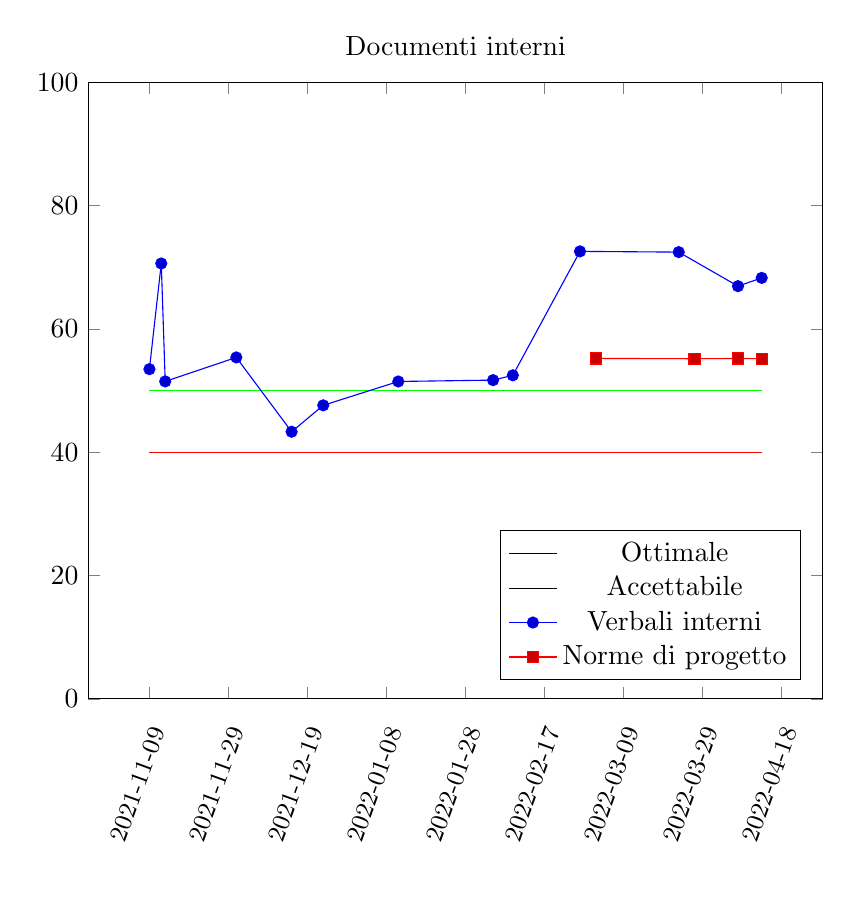
\begin{tikzpicture}
		\pgfplotsset{width=0.9\textwidth}
		\begin{axis}[
				title = {Documenti interni},
				axis x line = none,
				axis y line = none,
				ymin = 0, ymax = 100
			]
			\addplot [green]{50}; \label{opt}
			\addplot [red]{40}; \label{min}
		\end{axis}
		\begin{axis}[
				date coordinates in = x,
				xticklabel =	\year-\month-\day,
				x tick label style = {
						font = \small,
						text width = 1.9cm,
						align = center,
						rotate = 70,
						anchor = north east
					},
				ymin = 0, ymax = 100,
				legend pos = south east
			]
			\addlegendimage{/pgfplots/refstyle=opt}
			\addlegendentry{Ottimale}
			\addlegendimage{/pgfplots/refstyle=min}
			\addlegendentry{Accettabile}
			\addplot coordinates {
					(2021-11-09, 53.46)
					(2021-11-12, 70.60)
					(2021-11-13, 51.47)
					(2021-12-01, 55.36)
					(2021-12-15, 43.31)
					(2021-12-23, 47.59)
					(2022-01-11, 51.46)
					(2022-02-04, 51.68)
					(2022-02-09, 52.46)
					(2022-02-26, 72.56)
					(2022-03-23, 72.44)
					(2022-04-07, 66.92)
					(2022-04-13, 68.26)
				};\addlegendentry{Verbali interni}

			\addplot coordinates {
					(2022-03-02, 55.2)
					(2022-03-27, 55.15)
					(2022-04-07, 55.19)
					(2022-04-13, 55.15)
				};\addlegendentry{Norme di progetto}

		\end{axis}
	\end{tikzpicture}
\end{center}

\captionof{figure}{Leggibilità dei documenti interni nel tempo}

\clearpage
\begin{center}
	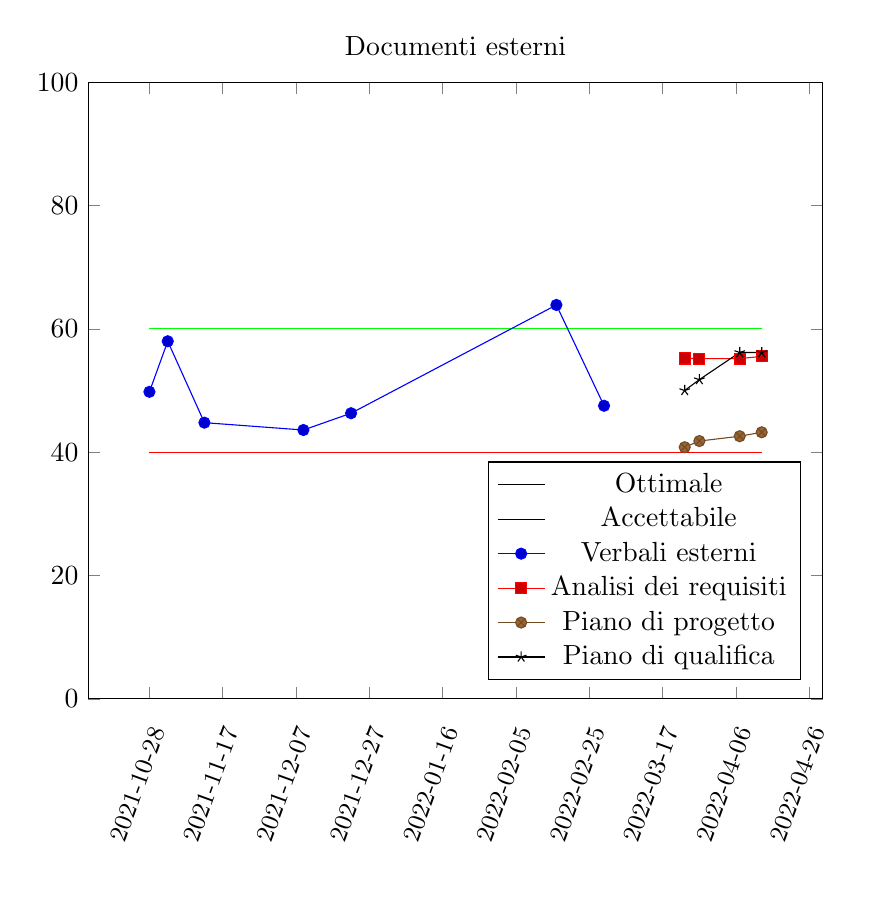
\begin{tikzpicture}
		\pgfplotsset{width=0.9\textwidth}
		\begin{axis}[
				title = {Documenti esterni},
				axis x line = none,
				axis y line = none,
				ymin = 0, ymax = 100
			]
			\addplot [green]{60}; \label{opt}
			\addplot [red]{40}; \label{min}
		\end{axis}
		\begin{axis}[
				date coordinates in = x,
				xticklabel =	\year-\month-\day,
				x tick label style = {
						font = \small,
						text width = 1.9cm,
						align = center,
						rotate = 70,
						anchor = north east
					},
				ymin = 0, ymax = 100,
				legend pos = south east
			]
			\addlegendimage{/pgfplots/refstyle=opt}
			\addlegendentry{Ottimale}
			\addlegendimage{/pgfplots/refstyle=min}
			\addlegendentry{Accettabile}
			\addplot coordinates {
					(2021-10-28, 49.78)
					(2021-11-02, 57.98)
					(2021-11-12, 44.78)
					(2021-12-09, 43.59)
					(2021-12-22, 46.31)
					(2022-02-16, 63.87)
					(2022-03-01, 47.52)
				};\addlegendentry{Verbali esterni}
			\addplot coordinates {
					(2022-03-23, 55.2)
					(2022-03-27, 55.16)
					(2022-04-07, 55.17)
					(2022-04-13, 55.53)
				};\addlegendentry{Analisi dei requisiti}

			\addplot coordinates {
					(2022-03-23, 40.8)
					(2022-03-27, 41.8)
					(2022-04-07, 42.58)
					(2022-04-13, 43.22)
				};\addlegendentry{Piano di progetto}

			\addplot coordinates {
					(2022-03-23, 50.00)
					(2022-03-27, 51.76)
					(2022-04-07, 56.17)
					(2022-04-13, 56.15)
				};\addlegendentry{Piano di qualifica}

		\end{axis}
	\end{tikzpicture}
\end{center}
\captionof{figure}{Leggibilità dei documenti esterni nel tempo}


\subparagraph{Riferimenti:} \underline{\href{http://www.corrige.it/leggibilita/lindice-gulpease/}{http://www.corrige.it/leggibilita/lindice-gulpease/}}

\subsection{Prodotti software}

\subsubsection{Copertura statement}
La metrica si basa sullo statement coverage.

\subparagraph{Prodotti coinvolti:}
\begin{center}
	\begin{tabularx}{\textwidth}{|X|X|X|}
		\hline
		\textbf{Prodotto} & \textbf{Valore accettabile } & \textbf{Valore ottimale } \\
		\hline
		Software          & $>$ 80\%                     & $>$ 95\%                     \\
		\hline
	\end{tabularx}\\[8pt]
	\mbox{}\\
\end{center}

\subparagraph{Strumenti utilizzati:} \begin{itemize}
	\item Jest;
	\item JSCoverage;
	\item PyTest;
	\item truffle.
\end{itemize}

\subparagraph{Struttura del grafico:}
Ogni punto indica la copertura percentuale degli statement nella data indicata.

\subparagraph{Andamento:}
\begin{center}
	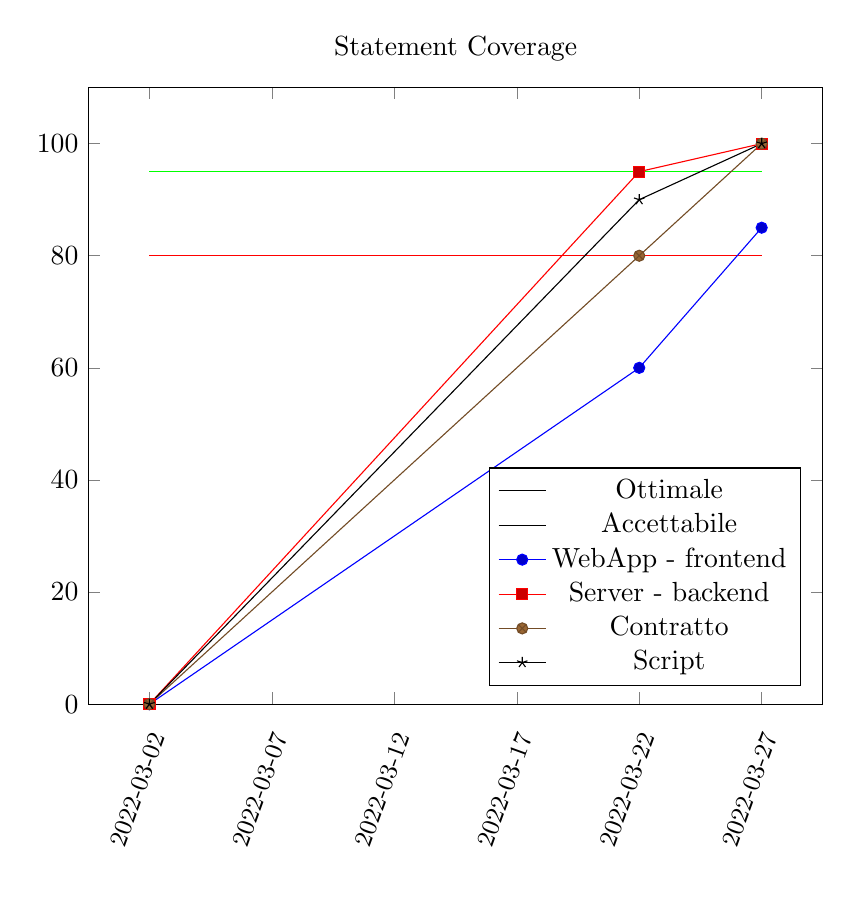
\begin{tikzpicture}
		\pgfplotsset{width=0.9\textwidth}
		\begin{axis}[
				title = {Statement Coverage},
				axis x line = none,
				axis y line = none,
				ymin = 0, ymax = 110
			]
			\addplot [green]{95}; \label{opt}
			\addplot [red]{80}; \label{min}
		\end{axis}
		\begin{axis}[
				date coordinates in = x,
				xticklabel =	\year-\month-\day,
				x tick label style = {
						font = \small,
						text width = 1.9cm,
						align = center,
						rotate = 70,
						anchor = north east
					},
				ymin = 0, ymax = 110,
				legend pos = south east
			]
			\addlegendimage{/pgfplots/refstyle=opt}
			\addlegendentry{Ottimale}
			\addlegendimage{/pgfplots/refstyle=min}
			\addlegendentry{Accettabile}
			\addplot coordinates {
					(2022-03-02, 0)
					(2022-03-22, 60)
					(2022-03-27, 85)
				};\addlegendentry{WebApp - frontend}
			\addplot coordinates {
					(2022-03-02, 0)
					(2022-03-22, 95)
					(2022-03-27, 100)
				};\addlegendentry{Server - backend}
			\addplot coordinates {
					(2022-03-02, 0)
					(2022-03-22, 80)
					(2022-03-27, 100)
				};\addlegendentry{Contratto}
			\addplot coordinates {
					(2022-03-02, 0)
					(2022-03-22, 90)
					(2022-03-27, 100)
				};\addlegendentry{Script}
		\end{axis}
	\end{tikzpicture}
\end{center}
\captionof{figure}{Copertura degli statement nel tempo}

\subsubsection{Copertura branch}
La metrica si basa sul branch coverage.

\subparagraph{Prodotti coinvolti:}
\begin{center}
	\begin{tabularx}{\textwidth}{|X|X|X|}
		\hline
		\textbf{Prodotto} & \textbf{Valore accettabile } & \textbf{Valore ottimale } \\
		\hline
		Software          & $>$ 80\%                     & $>$ 95\%                     \\
		\hline
	\end{tabularx}\\[8pt]
	\mbox{}\\
\end{center}

\subparagraph{Strumenti utilizzati:} \begin{itemize}
	\item Jest;
	\item JSCoverage;
	\item PyTest;
	\item truffle.
\end{itemize}

\subparagraph{Struttura del grafico:}
Ogni punto indica la copertura percentuale delle branch nella data indicata.

\subparagraph{Andamento:}
\begin{center}
	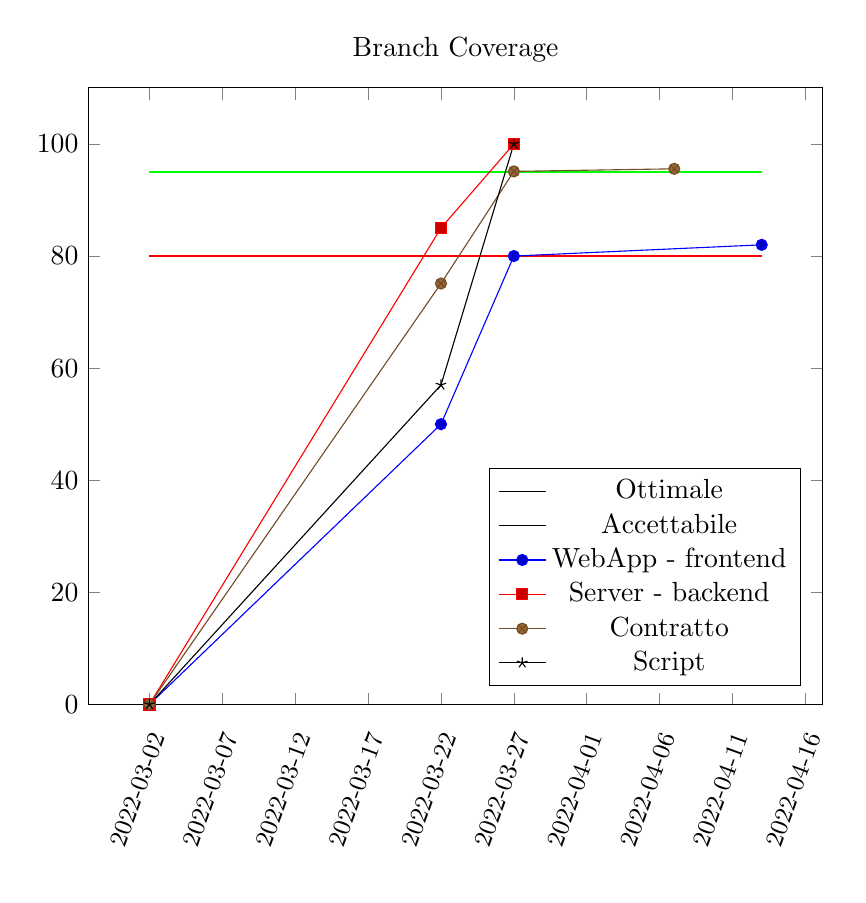
\begin{tikzpicture}
		\pgfplotsset{width=0.9\textwidth}
		\begin{axis}[
				title = {Branch Coverage},
				axis x line = none,
				axis y line = none,
				ymin = 0, ymax = 110
			]
			\addplot [green]{95}; \label{opt}
			\addplot [red]{80}; \label{min}
		\end{axis}
		\begin{axis}[
				date coordinates in = x,
				xticklabel =	\year-\month-\day,
				x tick label style = {
						font = \small,
						text width = 1.9cm,
						align = center,
						rotate = 70,
						anchor = north east
					},
				ymin = 0, ymax = 110,
				legend pos = south east
			]
			\addlegendimage{/pgfplots/refstyle=opt}
			\addlegendentry{Ottimale}
			\addlegendimage{/pgfplots/refstyle=min}
			\addlegendentry{Accettabile}
			\addplot coordinates {
					(2022-03-02, 0)
					(2022-03-22, 50)
					(2022-03-27, 80)
					(2022-04-13, 82)
				};\addlegendentry{WebApp - frontend}
			\addplot coordinates {
					(2022-03-02, 0)
					(2022-03-22, 85)
					(2022-03-27, 100)
				};\addlegendentry{Server - backend}
			\addplot coordinates {
					(2022-03-02, 0)
					(2022-03-22, 75.1)
					(2022-03-27, 95.1)
					(2022-04-07, 95.56)
				};\addlegendentry{Contratto}
			\addplot coordinates {
					(2022-03-02, 0)
					(2022-03-22, 57)
					(2022-03-27, 100)
				};\addlegendentry{Script}
		\end{axis}
	\end{tikzpicture}
\end{center}
\captionof{figure}{Copertura delle branch nel tempo}

\clearpage
\section{Qualità di processo}
\subsubsection{Time variance}
La metrica si basa sulla variazione percentuale rispetto alla stima iniziale.

\subparagraph{Prodotti coinvolti:}
\begin{center}
	\begin{tabularx}{\textwidth}{|X|X|X|}
		\hline
		\textbf{Prodotto} & \textbf{Valore accettabile } & \textbf{Valore ottimale } \\
		\hline
		Software          & $<$ 20\%                     & 0\%                       \\
		\hline
		Documentazione    & $<$ 20\%                     & 0\%                       \\
		\hline
	\end{tabularx}\\[8pt]
	\mbox{}\\
\end{center}

\subparagraph{Struttura del grafico:}
Ogni punto indica la variazione del consuntivo rispetto al preventivo di un ciclo di sprint.

\subparagraph{Andamento:}
\begin{center}
	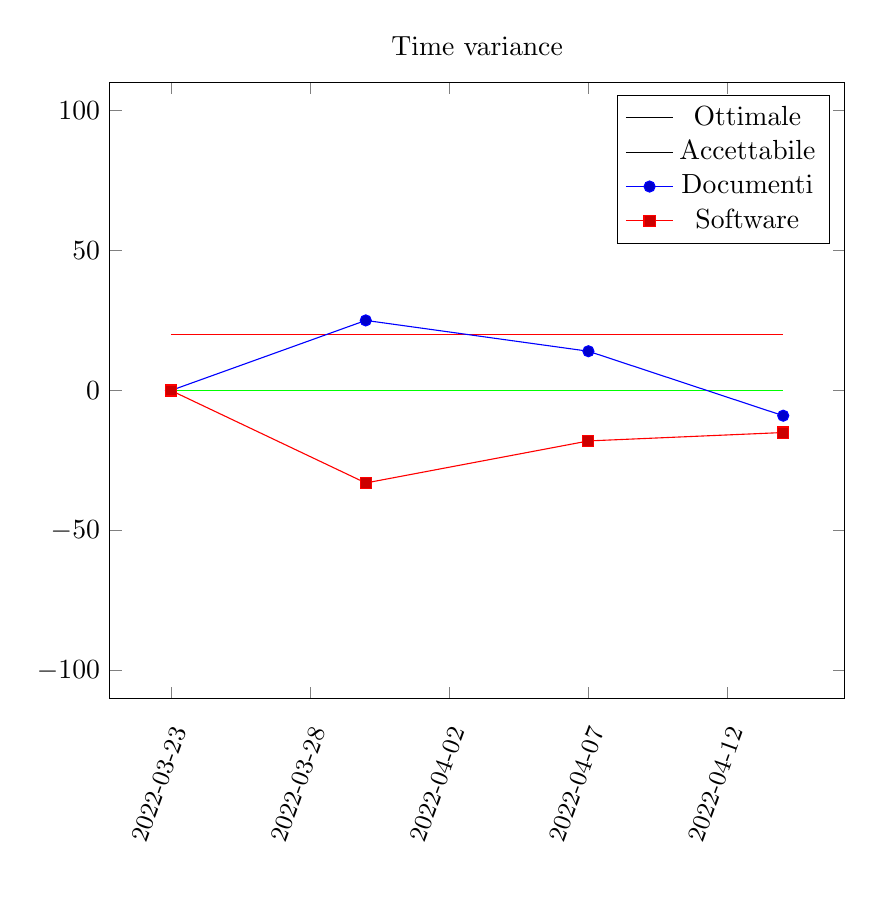
\begin{tikzpicture}
		\pgfplotsset{width=0.9\textwidth}
		\begin{axis}[
				title = {Time variance},
				axis x line = none,
				axis y line = none,
				ymin = -110, ymax = 110
			]
			\addplot [green]{0}; \label{opt}
			\addplot [red]{20}; \label{min}
		\end{axis}
		\begin{axis}[
				date coordinates in = x,
				xticklabel =	\year-\month-\day,
				x tick label style = {
						font = \small,
						text width = 1.9cm,
						align = center,
						rotate = 70,
						anchor = north east
					},
				ymin = -110, ymax = 110
			]
			\addlegendimage{/pgfplots/refstyle=opt}
			\addlegendentry{Ottimale}
			\addlegendimage{/pgfplots/refstyle=min}
			\addlegendentry{Accettabile}
			\addplot coordinates {
					(2022-03-23, 0)
					(2022-03-30, +25)
					(2022-04-07, +14)
					(2022-04-14, -9)
				};\addlegendentry{Documenti}
			\addplot coordinates {
					(2022-03-23, 0)
					(2022-03-30, -33)
					(2022-04-07, -18)
					(2022-04-14, -15)
				};\addlegendentry{Software}
		\end{axis}
	\end{tikzpicture}
\end{center}
\captionof{figure}{Rispetto delle scadenze temporali nel tempo}

\clearpage
\subsubsection{Budget variance}
La metrica si basa sulla variazione percentuale rispetto alla stima iniziale.

\subparagraph{Prodotti coinvolti:}
\begin{center}
	\begin{tabularx}{\textwidth}{|X|X|X|}
		\hline
		\textbf{Prodotto} & \textbf{Valore accettabile } & \textbf{Valore ottimale } \\
		\hline
		Software          & $<$ 20\%                     & 0\%                       \\
		\hline
		Documentazione    & $<$ 20\%                     & 0\%                       \\
		\hline
	\end{tabularx}\\[8pt]
	\mbox{}\\
\end{center}

\subparagraph{Struttura del grafico:}
Ogni punto indica la variazione del consuntivo rispetto al preventivo di un ciclo di sprint.

\subparagraph{Andamento:}
\begin{center}
	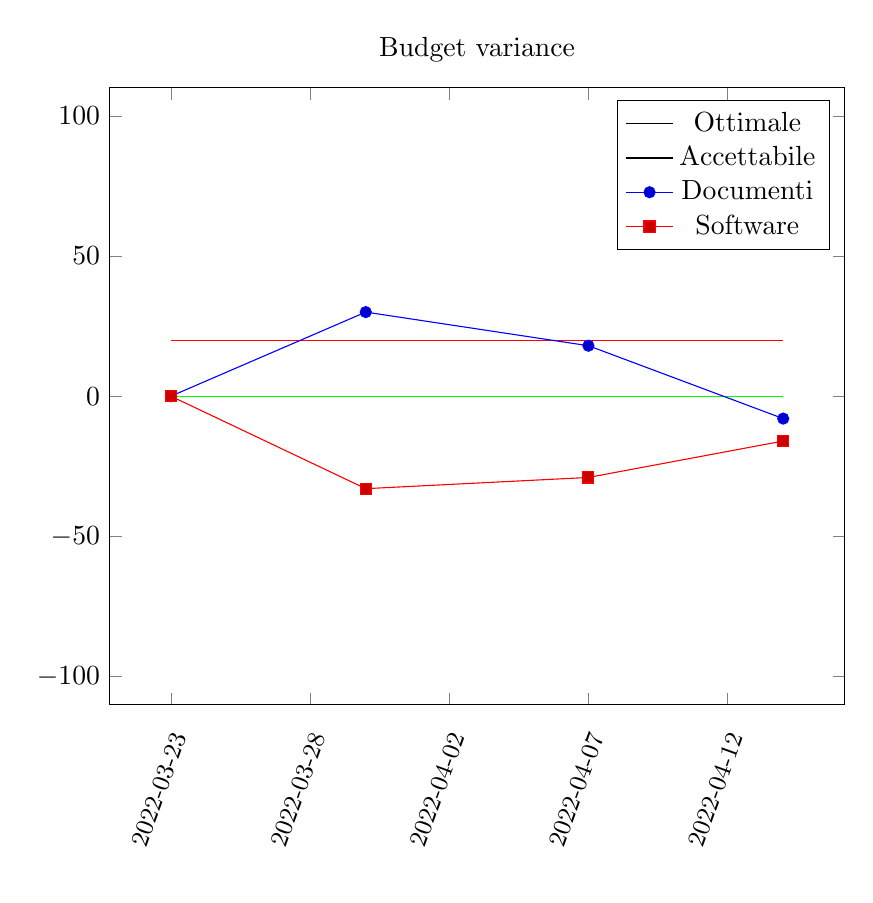
\begin{tikzpicture}
		\pgfplotsset{width=0.9\textwidth}
		\begin{axis}[
				title = {Budget variance},
				axis x line = none,
				axis y line = none,
				ymin = -110, ymax = 110
			]
			\addplot [green]{0}; \label{opt}
			\addplot [red]{20}; \label{min}
		\end{axis}
		\begin{axis}[
				date coordinates in = x,
				xticklabel =	\year-\month-\day,
				x tick label style = {
						font = \small,
						text width = 1.9cm,
						align = center,
						rotate = 70,
						anchor = north east
					},
				ymin = -110, ymax = 110
			]
			\addlegendimage{/pgfplots/refstyle=opt}
			\addlegendentry{Ottimale}
			\addlegendimage{/pgfplots/refstyle=min}
			\addlegendentry{Accettabile}
			\addplot coordinates {
					(2022-03-23, 0)
					(2022-03-30, +30)
					(2022-04-07, +18)
					(2022-04-14, -8)
				};\addlegendentry{Documenti}
			\addplot coordinates {
					(2022-03-23, 0)
					(2022-03-30, -33)
					(2022-04-07, -29)
					(2022-04-14, -16)
				};\addlegendentry{Software}
		\end{axis}
	\end{tikzpicture}
\end{center}
\captionof{figure}{Rispetto delle budget economico nel tempo}

\end{document}
